
%(BEGIN_QUESTION)
% Copyright 2005, Tony R. Kuphaldt, released under the Creative Commons Attribution License (v 1.0)
% This means you may do almost anything with this work of mine, so long as you give me proper credit

Calculate all voltage drops and currents in this circuit, complete with arrows for current direction and polarity markings for voltage polarity.  Then, calculate the overall voltage gain of this amplifier circuit ($A_V$), both as a ratio and as a figure in units of decibels (dB):

$$\includegraphics[width=15.5cm]{i01474x01.eps}$$

\underbar{file i01474}
%(END_QUESTION)





%(BEGIN_ANSWER)

$$\includegraphics[width=15.5cm]{i01474x02.eps}$$

$A_V$ = 1.468 = 3.335 dB

%(END_ANSWER)





%(BEGIN_NOTES)

Operational amplifier circuits provide a great opportunity to review basic concepts of DC circuits: voltage drops, polarity, current directions, Ohm's Law, Kirchhoff's Voltage Law, Kirchhoff's Current Law, etc.  This circuit is no exception.  Emphasize the fact that a great many opamp circuits may be comprehensively analyzed merely with knowledge of these fundamental principles and the characteristics of an ideal opamp (zero input current, infinite open-loop gain, unlimited output voltage swing, zero voltage between input terminals when negative feedback is in effect).

Some students may arrive at the wrong gain figure because they blindly followed a formula with $R_1$ and $R_2$ shown as variables, plugging in this circuit's values for $R_1$ and $R_2$ without considering which resistor is which (is $R_1$ the feedback resistor or is $R_2$?).  This is by design, as I want students to learn to {\it think} about what they are doing rather than thoughtlessly follow instructions.

%INDEX% Electronics review: opamp noninverting amplifier circuit

%(END_NOTES)


